\documentclass[12pt, a4paper, oneside]{ctexart}

\usepackage{amsmath}
\usepackage{amssymb}
\usepackage{bm}
\usepackage{graphicx}
\usepackage{mathrsfs}
\usepackage{geometry}
\usepackage{framed}
\usepackage{color}
\usepackage{listings}
\usepackage{fancyhdr}
\usepackage{booktabs}
\usepackage{makecell}
\usepackage{indentfirst}
\usepackage{authblk}
\usepackage{multicol}
% \usepackage{draftwatermark}       % 需要应用水印时取消注释
\usepackage{enumitem}
\usepackage[hidelinks]{hyperref}
\usepackage{tikz}
\usetikzlibrary{positioning, shapes.geometric}

% 分栏线宽
\columnseprule=0.4pt

% 定制第二级无序列表的点样式
\setlist[itemize,2]{label=$\diamond$}

\pagestyle{fancy}

\fancyhf{}      % 清空页眉页脚设置
\fancyhead[L] {
    % 工大计算机系logo
    
\includegraphics[height=7mm]{./images/logo1.jpg}
}
\fancyhead[C]{《操作系统》复习}
\fancyhead[R]{\leftmark}    % 右侧页眉:当前章标题

% 页脚居中放置页码
\fancyfoot[C]{\thepage}

% 设置章节标题自动编号的格式
\ctexset{
  section/number=\chinese{section},
%   subsection/name={,},
%   subsection/number=\chinese{subsection}
}

\lstset{
  language=pascal,
  basicstyle=\ttfamily,
  frame=single,
  numbers=left
}

% \SetWatermarkText{Eslzzyl整理}            % 设置水印内容
% \SetWatermarkLightness{0.9}             % 设置水印透明度 0-1
% \SetWatermarkScale{0.8}                   % 设置水印大小 0-1

\renewcommand{\headrulewidth}{1pt}  %页眉线宽,设为0可以去页眉线
\renewcommand{\footrulewidth}{1pt}  %脚注线的宽度

\definecolor{shadecolor}{RGB}{241, 241, 255}

\title{
    
\includegraphics[width=0.3\textwidth]{images/hfut-badge.pdf}
    
    \vspace{20pt}
    《操作系统》总复习
}
\author{Eslzzyl}
\date{\today}

\newcounter{problemname}
\newenvironment{problem}{\begin{shaded}\stepcounter{problemname}\par\noindent\textbf{例题\arabic{problemname}. }}{\end{shaded}\par}
\newenvironment{solution}{\begin{shaded}\par\noindent\textbf{解答:}}{\end{shaded}\par}
% \newenvironment{solution}{\par\noindent\textbf{答案. }}{\par}
\newenvironment{note}{\par\noindent\textbf{例题\arabic{problemname}的注记. }}{\\\par}

\begin{document}

\maketitle
\newpage
\tableofcontents
\vspace{20pt}
考试题型
\begin{itemize}
    \item 主观题 50\%:简答、计算、问答
    \item 客观题 50\%:单选、填空、判断
\end{itemize}
\vspace{20pt}
本材料的内容排布原则:以课本章节编号为准,只列出PPT有的内容

\newpage

\section{操作系统引论}

操作系统的\textbf{定义}:操作系统是一组管理和控制计算机软件和硬件资源,合理
组织计算机系统工作流程,以及方便用户使用的程序的集合。

\subsection{操作系统的目标和作用}

\subsubsection{操作系统的目标}

\begin{itemize}
    \item 方便性:使计算机更易使用
    \item 有效性:使资源利用更高效
    \item 可扩充性
    \item 开放性
\end{itemize}

\subsubsection{操作系统的作用}

\begin{itemize}
    \item 作为用户与计算机硬件系统之间的接口
    \item 作为计算机系统资源的管理者
    \item 实现对计算机资源的抽象
\end{itemize}

\subsection{操作系统的发展过程}

推动OS发展的主要动力:
\begin{itemize}
    \item 不断提高计算机资源利用率
    \item 方便用户
    \item 器件的不断更新换代
    \item 计算机体系结构的发展
    \item 不断提出新的应用需求
\end{itemize}

\subsubsection{无操作系统时代}

对计算机的所有操作采用人工操作方式完成。人工操作方式的缺点:
\begin{itemize}
    \item 用户独占全机
    \item CPU等待人工操作
\end{itemize}

由于以上两点,昂贵的机器资源在大部分时间内处于空闲状态,非常浪费。

优点:交互性好,即用户可以得到机器的立即响应。

\subsubsection{单道批处理系统}

\textbf{批处理系统}:在计算机上加载一个专门监控软件,在其控制下,计算机
能够自动地、成批地处理一个或多个用户的一批作业。

批处理系统的特点:
\begin{itemize}
    \item 系统吞吐量大
    \item 资源利用率高
    \item 平均周转时间短
    \item 无交互能力(缺点)
\end{itemize}
 fd
\textbf{单道批处理系统}:先把一批作业输入到磁带上,在监控程序的控制下使这批作业一个接一个地处理。
内存中始终只保持一道作业。

代表系统:IBM的FMS(Fortran Monitoring System),1960s

一定程度上改善了资源浪费,但失去了交互性。单个程序独占系统,程序IO时CPU空等。

单道批处理系统的特点:自动性、顺序性、单道性

\subsubsection{多道批处理系统}

出现的动力是希望提高资源利用率和系统吞吐量。

代表系统(也是第一个):IBM的OS/360,1960s

由作业调度程序按照一定的算法,从后备队列中选择若干个作业调入内存,使它们共享CPU资源。

相比单道批处理系统,多道批处理系统的资源利用率更高,但仍然没有交互性。

特点:多道性、无序性、调度性

\subsubsection{分时系统}

出现的动力是改善交互性。

分时系统:在一台主机上连接若干个终端,允许多个用户通过终端以交互方式共享主机资源。

代表系统:CTSS(1962)、Multics(1964)

特点:
\begin{itemize}
    \item 多路性:众多联机用户可以同时使用同一台计算机
    \item 独立性:各终端用户感觉到自己独占了计算机
    \item 及时性:用户的请求能在很短时间内得到响应
    \item 交互性:用户与计算机之间可进行“会话”
\end{itemize}

\subsubsection{实时系统}

实时计算:系统的正确性不仅由计算的逻辑结果来确定,而且还取决于产生结果的时间。

常见的实时系统:
\begin{itemize}
    \item 工业控制系统、武器控制系统
    \item 信息查询系统
    \item 多媒体系统
    \item 嵌入式系统
\end{itemize}

代表系统:WinCE,嵌入式Linux,ucOSII,VxWorks等

特点:实时性、高安全性、高可靠性(效率放第二位)、整体性强、会话能力要求不高

\subsection{操作系统的基本特性}

四大基本特征
\begin{itemize}
    \item 并发(Concurrence)
    \item 共享(Sharing)
    \item 虚拟(Virtual)
    \item 异步(Asynchronism)
\end{itemize}

\subsubsection{并发}

\begin{itemize}
    \item 并行性:多个事件在同一时刻发生
    \item 并发性:多个事件在同一时间间隔内发生
\end{itemize}

单处理机可以实现并发(宏观上并发,微观上分时运行),多处理机可以实现并行。

\subsubsection{共享}

即:系统中的资源可供内存中多个并发执行的进程共同使用。

资源共享方式:
\begin{itemize}
    \item 互斥共享方式:如打印机、磁带机
    \item 同时访问方式:如磁盘、内存
\end{itemize}

并发和共享是多用户OS的最基本特征。

\subsubsection{虚拟}

指通过某种技术把一个物理实体变为若干个逻辑上的对物。

\subsubsection{异步}

进程的异步性:进程是以人们不可预知的速度向前推进的。进程的执行通常都不是“一气呵成”的,而是“停停走走”

\subsection{操作系统的主要功能}

\begin{multicols}{2}
\begin{itemize}
    \item 处理机管理功能
    \begin{itemize}
        \item 进程控制
        \item 进程同步
        \item 进程通信
    \end{itemize}
    \item 存储器管理功能
    \begin{itemize}
        \item 内存分配
        \item 内存保护
        \item 地址映射
        \item 内存扩充
    \end{itemize}
    \item 设备管理功能
    \begin{itemize}
        \item 缓冲管理
        \item 设备分配
        \item 设备处理
    \end{itemize}
    \item 文件管理功能
    \begin{itemize}
        \item 文件存储空间的管理
        \item 目录管理
        \item 文件的读写管理和保护
    \end{itemize}
    \item 操作系统接口
    \begin{itemize}
        \item 用户接口
        \item 程序接口
    \end{itemize}
\end{itemize}
\end{multicols}

\subsection{操作系统结构}

\subsubsection{无结构OS}

基本上没有优点。
\begin{itemize}
    \item 操作系统庞大杂乱,缺乏清晰的程序结构
    \item 操作系统的编写、调试、维护复杂,保证操作系统程序的正确困难
\end{itemize}

\subsubsection{模块化结构OS}

优点:
\begin{itemize}
    \item 提高OS设计的正确性、可理解性和可维护性
    \item 增强OS的可移植性, 加速OS的开发过程
\end{itemize}

缺点:
\begin{itemize}
    \item 结构划分和接口设计困难
    \item 模块之间调用关系复杂,牵一发而动全身
\end{itemize}

\subsubsection{分层式结构OS}

原则:将功能模块分层,层内模块可以互相调用,层间模块只允许高层调用它下面紧邻着的那层,不允许反过来。

将最靠近硬件的低层OS部分称为操作系统内核,内核通常常驻主存。

优点:
\begin{itemize}
    \item 容易保证系统的正确性。
    \item 容易扩充、维护和移植。
\end{itemize}

缺点:效率低下。

\subsubsection{微内核OS}

将OS划分为两大部分:
\begin{itemize}
    \item 内核,只提供客户-服务器通信机制和与硬件紧密相关的较基本的功能
    \item 提供各类服务的一组服务器进程
\end{itemize}

OS采用C/S模式提供各类操作系统服务。

优点:
\begin{itemize}
    \item 灵活、容易移植、容易扩展、可靠
    \item 支持分布式系统
\end{itemize}

缺点:还是效率低下。

\newpage

\section{进程管理}

\subsection{前趋图和程序执行}

\subsubsection{前趋图}

前趋图:用于描述实体(进程、程序段)之间执行次序的DAG。每个结点表示一个进程或程序段,乃至一条语句。
结点之间的有向边表示两个结点之间存在偏序或前趋关系。

把没有前趋的结点成为初始结点,把没有后继的结点称为终止结点。

\subsubsection{程序的顺序执行}

特征:
\begin{itemize}
    \item 顺序性:一个操作做完之后才进行下一个操作
    \item 封闭性:一旦开始执行,其结构不受外界因素影响
    \item (结果的)可再现性
\end{itemize}

\subsubsection{程序的并发执行}

只有不存在前趋关系的程序之间才有可能并发执行。

特征:
\begin{itemize}
    \item 间断性
    \item 失去封闭性
    \item 不可再现性
\end{itemize}

\subsection{进程的描述}

\subsubsection{进程的定义和特征}

(传统OS中)进程的\textbf{定义}:进程是进程实体的运行过程,是系统进行资源分配和调度的一个独立单位。

进程实体:程序段+相关的数据段+PCB

进程的特征:
\begin{itemize}
    \item 动态性:进程有生命周期,而程序只是一组有序指令的集合,是静态的。
    \item 并发性:指多个进程可以同时存在于内存中,且能在一段时间内同时运行。
    \item 独立性:进程实体是一个能独立运行、独立获得资源和独立接受调度的基本单位。
    \item 异步性:进程按照各自独立的、不可预知的速度向前推进。
\end{itemize}

\subsubsection{进程的基本状态及转换}

三种基本状态:
\begin{itemize}
    \item 就绪(Ready)状态:进程已经得到除了CPU之外的所有资源,一旦得到CPU就立即开始执行。
    \item 执行(Running)状态:单处理机系统中只有一个进程处于执行状态,多处理机系统中有多个进程处于执行状态。
    \item 阻塞(Blocking)状态:指正在执行的进程由于发生某事件为暂时无法继续执行的状态。此时会引发进程调度。
\end{itemize}

三种基本状态的转换:参见课本P40 图2-5

\subsubsection{PCB}

OS管理的数据结构:
\begin{itemize}
    \item 内存表
    \item 设备表
    \item 文件表
    \item 进程表
\end{itemize}

进程表就是PCB。本节只介绍PCB。

PCB进程存在的唯一标志。

\begin{multicols}{2}
PCB中的内容:
\begin{itemize}
    \item 进程标识符
    \item 处理机状态
    \item 进程调度信息
    \item 进程控制信息
\end{itemize}

PCB的组织方式:
\begin{itemize}
    \item 线性方式
    \item 链接方式
    \item 索引方式
\end{itemize}
\end{multicols}

\subsection{进程控制}

待补

\subsection{进程同步}

\subsubsection{进程同步的基本概念}

两种形式的制约关系:
\begin{itemize}
    \item 间接相互制约关系:共享临界资源引起
    \item 直接相互制约关系:直接依赖引起
\end{itemize}

临界资源:一次仅能为一个进程所使用的资源。

实例:
\begin{itemize}
    \item 硬件资源:打印机
    \item 软件资源:所有\textbf{变}量、指针、数组等
\end{itemize}

临界区:每个进程中访问临界资源的那部分代码。

临界区访问控制模型:在临界区前面加入代码(进入区),在临界区后也加入代码(退出区)

同步机制应遵循的原则:
\begin{enumerate}
    \item \label{kxrj}空闲让进:当无进程处于临界区时,请求进入临界区的进程可立即进入
    \item \label{mzdd}忙则等待:当已有进程进入临界区时,其他试图进入临界区进程须等待
    \item \label{yxdd}有限等待:对要求访问临界资源进程,保证能在有限时间内进入临界区
    \item \label{rqdd}让权等待:当进程不能进入临界区时,应释放处理机
\end{enumerate}

其中\ref{kxrj}和\ref{mzdd}是必须实现的,否则无法实现互斥;
\ref{yxdd}和\ref{rqdd}不实现不会影响互斥,但会严重影响系统的性能。

解决同步问题的方法:
\begin{itemize}
    \item 软件方法:如Peterson算法
    \item 硬件方法:
    \begin{itemize}
        \item 关中断
        \item 利用Test-and-Set指令
        \item 利用Swap指令
    \end{itemize}
\end{itemize}

早期的进程同步软件方法:
\begin{itemize}
    \item 按需访问:违背忙则等待、有限等待、让权等待
    \item 轮询:违背让权等待、有限等待,同时严格限制了资源访问顺序
    \item 访前先看:违背空闲让进、有限等待、让权等待
\end{itemize}

\subsubsection{信号量机制}

1965年荷兰学者Dijkstra提出。

整数型信号量:
\begin{itemize}
    \item 定义整数信号量S,表示可用资源数量
    \item 定义两个原子操作:wait/signal(P/V)
    \item 在critical section前后使用wait(S)和signal(S)
\end{itemize}

\begin{lstlisting}
    VAR S:integer := 1;
    function Wait ( var S: integer )
    Begin
        while ( S <= 0 );
        S := S-1;
    end

    function Signal( var S : integer )
    Begin
        S := S+1;
    end
\end{lstlisting}

记录型信号量:
\begin{itemize}
    \item 定义S和wait/signal同上
    \item 进程无法访问临界资源时,阻塞自身;释放临界资源时,如果有进程还在阻塞,则唤醒该进程。
\end{itemize}

\begin{lstlisting}
    type semaphore = record
        value: integer;     // 资源数量
        L: list of process; // 阻塞进程队列
    end

    function wait (var S : Semaphore)
    Begin
        S.value := S.value-1;
        if ( S.value < 0 ) then block (S.L);
    end

    function signal(var S : Semaphore)
    Begin
        S.value := S.value+1;
        if ( S.value <= 0 ) then wakeup (S.L);
    end
\end{lstlisting}

\begin{itemize}
    \item S.value >= 0时,表示资源数量。
    \item S.value < 0时,其绝对值表示被阻塞进程的数量。
\end{itemize}

\subsection{经典的进程同步问题}

\subsubsection{生产者-消费者问题}

单生产者单消费者、多缓冲:
\begin{lstlisting}
    VAR mutex, empty, full: semaphore := 1, n, 0 ;
        in,out: integer := 0, 0 ;
        Buffer: array [0..n-1] of item ;
    Parbegin
        Producer:
        begin
            repeat
                produce an item in nextp ;
                wait( empty ) ;
                wait( mutex ) ;
                Buffer(in) := nextp ;
                in := (in + 1 ) mod n ;
                signal( mutex ) ;
                signal( full ) ;
            until false
        end
        Consumer:
        begin
            repeat
                wait( full ) ;
                wait( mutex ) ;
                nextc = Buffer(out);
                out := (out + 1 ) mod n ;
                signal( mutex ) ;
                signal( empty ) ;
                consume the item nextc ;
            until false
        end
    Parend
\end{lstlisting}

多生产者多消费者、单缓冲:删去上面代码的mutex。

单生产者单消费者、单缓冲:删去上面代码的mutex,将empty的初值改成1。

允许生产者写时,消费者可读:
\begin{lstlisting}
    VAR mutexC, mutexP, empty, full: semaphore := 1,1, n, 0 ;
        in,out: integer := 0, 0 ;
        Buffer: array [0..n-1] of item ;
    Parbegin
        Producer:
        begin
            repeat
                produce an item in nextp ;
                wait( empty ) ;
                wait( mutexP ) ;
                Buffer(in) := nextp ;
                in := (in + 1 ) mod n ;
                signal( mutexP ) ;
                signal( full ) ;
            until false
        end
        Consumer:
        begin
            repeat
                wait( full ) ;
                wait( mutexC ) ;
                nextc = Buffer(out);
                out := (out + 1 ) mod n ;
                signal( mutexC ) ;
                signal( empty ) ;
                consume the item nextc ;
            until false
        end
    Parend
\end{lstlisting}

缓冲池无限大:
\begin{lstlisting}
    VAR mutex, full: semaphore := 1, 0 ;
        in,out: integer := 0, 0 ;
        Buffer: array [0..n-1] of item ;
    Parbegin
        Producer:
        begin
            repeat
                produce an item in nextp ;
                wait( mutex ) ;
                Buffer(in) := nextp ;
                in := (in + 1 ) mod n ;
                signal( mutex ) ;
                signal( full ) ;
            until false
        end
        Consumer:
        begin
            repeat
                wait( full ) ;
                wait( mutex ) ;
                nextc = Buffer(out);
                out := (out + 1 ) mod n ;
                signal( mutex ) ;
                consume the item nextc ;
            until flase
        end
    Parend
\end{lstlisting}

\subsubsection{读者-写者问题}

允许多个读者同时访问资源,写者写时不允许其他进程读或写。

\begin{lstlisting}
    VAR rmutex,wmutex: semaphore := 1, 1 ;
        readcount: integer := 0 ;
    Parbegin
        Reader:
        begin
            repeat
                wait( rmutex ) ;
                if ( readcount = 0 ) wait( wmutex ) ;
                readcount := readcount + 1 ;
                signal( rmutex ) ;
                perform read operation ;
                wait( rmutex ) ;
                readcount := readcount - 1 ;
                if ( readcount = 0 ) signal( wmutex ) ;
                signal( rmutex ) ;
            until false
        end
        Writer:
        begin
            repeat
                wait( wmutex ) ;
                perform write operation;
                signal( wmutex ) ;
            until flase
        end
    Parend
\end{lstlisting}

\subsubsection{哲学家进餐问题}

\begin{lstlisting}
    VAR chopsticks: array [0..4] of semaphore := 1,1,1,1,1 ;
    Parbegin
        philosopher0-3:
        begin
            repeat
                wait( chopsticks[ i ] ) ;
                wait( chopsticks[ (i+1) mod 5 ] );
                eat ;
                signal( chopsticks[ i ] ) ;
                signal( chopsticks[ (i+1) mod 5 ] );
                think
            until false
        end
        philosopher4:
        begin
            repeat
                wait( chopsticks[ (i+1) mod 5 ] );
                wait( chopsticks[ i ] ) ;
                eat ;
                signal( chopsticks[ i ] ) ;
                signal( chopsticks[ (i+1) mod 5 ] );
                think
            until false
        end
    Parend
\end{lstlisting}

原则:按序申请资源

\subsubsection{理发师问题}

上课没讲,说是课后思考

\subsection{进程通信}

\subsubsection{共享存储器系统}

分类
\begin{itemize}
    \item 基于共享数据结构的通信方式
    \item 基于共享存储区的通信方式
\end{itemize}

特点
\begin{itemize}
    \item 适合大量的数据快速交换
    \item 程序员负担重
\end{itemize}

\subsubsection{管道通信系统}

通过一个固定大小的共享文件实现通信。UNIX首创。

\subsubsection{消息通信系统}

当前应用最广泛。

分类:
\begin{itemize}
    \item 直接通信方式
    \item 间接通信方式:通过信箱(mailbox)通信
    \begin{itemize}
        \item 公有信箱
        \item 私有信箱
        \item 共享信箱
    \end{itemize}
\end{itemize}

特点:
\begin{itemize}
    \item 操作系统隐藏通信细节
    \item 通信程序简单
    \item 可以跨网络传输
    \item 灵活
\end{itemize}

\subsection{线程的基本概念}

\subsubsection{线程的引入}

传统进程的两个基本属性
\begin{itemize}
    \item 是拥有资源的独立单位
    \item 是调度和分派的基本单位
\end{itemize}

线程的特点:
\begin{itemize}
    \item 是能独立运行的基本单位,且切换代价远小于进程。
    \item 线程不拥有系统资源,而是仅拥有一点必不可少的、能保证独立运行的资源。
    \item 多个线程可以共享一个进程的资源
\end{itemize}

\subsection{线程的实现}

\subsubsection{内核支持线程KST}

在内核的支持下运行。调度以线程为单位进行。

\subsubsection{用户级线程ULT}

无须内核支持,与内核无关,甚至内核不知道此类线程的存在。调度以进程为单位进行。

\newpage
\section{处理机调度与死锁}

\subsection{处理机调度的层次和调度算法的目标}

\subsubsection{处理机调度的层次}

\begin{itemize}
    \item 高级调度:又称长程调度、作业调度、接纳调度。
    \begin{itemize}
        \item 调度对象是作业。
        \item 根据某种算法,决定将外存上处于后备队列中的哪几个作业调入内存。
        \item 设置在多道批处理系统中。分时系统和实时系统不设置。
        \item 调度频率低,典型时间:几分钟。
        \item 因为调度频率低,调度算法可以设计得很复杂。
    \end{itemize}
    \item 低级调度:又称进程调度或短程调度。
    \begin{itemize}
        \item 调度对象是就绪的进程或内核级线程。
        \item 根据某种算法,决定就绪队列中的哪个进程获得处理机。
        \item 这是最基本的调度方式,在各类OS中都必须设置。
        \item 调度频率高,典型时间:几十毫秒。
        \item 因为调度时间短,调度算法必须足够简单。
    \end{itemize}
    \item 中级调度:又称内存调度。
    \begin{itemize}
        \item 调度对象是就绪进程和阻塞进程。
        \item 其实就是内存对换功能。引入的主要目的是提高内存利用率和系统吞吐量。
    \end{itemize}
\end{itemize}

\subsubsection{处理机调度算法的目标}

\begin{itemize}
    \item 面向用户的准则
    \begin{itemize}
        \item 响应时间快
        \item 截止时间有保证
    \end{itemize}
    \item 面向系统的准则
    \begin{itemize}
        \item 系统吞吐量高
        \item 处理机利用率高
        \item 资源利用均衡
    \end{itemize}
\end{itemize}

\begin{problem}
单选:进程调度的准则不能是(\ \ )
\begin{enumerate}
    \item [A. ] 最大的内存利用率
    \item [B. ] 最短的周转时间
    \item [C. ] 最大的CPU利用率
    \item [D. ] 最短的等待时间
\end{enumerate}
\end{problem}

\begin{solution}
    A
\end{solution}

\subsubsection{周转时间}

周转时间:从作业被提交给系统开始,到作业完成为止的时间。=等待时间+执行时间

设$T_i$是第$i$个作业的周转时间,$n$为作业总数,则系统的平均周转时间定义为
\begin{equation}
    T=\frac{1}{n}\left[\sum_{i=1}^{n}T_i\right]
\end{equation}

再设$T_{si}$是第$i$个作业的要求服务时间,则系统的平均带权周转时间定义为
\begin{equation}
    W=\frac{1}{n}\left[\sum_{i=1}^{n}\frac{T_i}{T_{si}}\right]
\end{equation}

\subsection{作业与作业调度}

\subsubsection{先来先服务(FCFS)调度算法}

FCFS(first-come, first-served)是最简单的调度算法。即可用于作业调度,也可用于进程调度。

特点:
\begin{itemize}
    \item 实现简单
    \item 对短作业不公平
\end{itemize}

\subsubsection{短作业/短进程优先(SJF/SPF)调度算法}

SJF(short job first)、SPF(short process first)

以作业要求的服务时间长短计算优先级。作业越短,优先级越高。

特点:
\begin{itemize}
    \item 实现困难,因为难以估计作业的执行时间。
    \item 有利于短作业。
    \item 对长作业不公平。
\end{itemize}

\subsubsection{优先级调度算法(PSA)}
\label{PSA}

PSA(priority-scheduling algorithm)

由外部赋予作业相应的优先级,根据该优先级调度。高优先级作业优先运行。

\subsubsection{高响应比优先调度算法(HRRN)}

HRRN(Highest Response Ratio Next)

基本思想是动态优先级,作业等待时间越长,优先级越高。

\begin{equation*}
    \text{响应比}R_p=\frac{\text{等待时间+要求服务时间}}{\text{要求服务时间}}=\frac{\text{响应时间}}{\text{要求服务时间}}
\end{equation*}

以响应比作为优先级。

特点:
\begin{itemize}
    \item 既照顾了短作业,又考虑了作业到达的先后次序,不会使长作业长期得不到服务。
    \item 每次调度之前要计算响应比,系统开销加大。
\end{itemize}

\begin{problem}
    5个进程A,B,C,D,E分别于0,1,2,3,4时刻到达系统,要求服务时间分别为4,3,5,2,4, 请计算:
    \begin{enumerate}
        \item [(1). ] 采用FCFS时进程执行顺序和平均周转时间;
        \item [(2). ] 采用SPF时进程执行顺序和平均周转时间;
        \item [(3). ] 采用HRRN时进程执行顺序和平均周转时间。
    \end{enumerate}
\end{problem}

\begin{solution}
    \begin{enumerate}
        \item [(1). ]
        进程执行顺序:A$\rightarrow$B$\rightarrow$C$\rightarrow$D$\rightarrow$E\\
        平均周转时间:T = (4+6+10+11+14) / 5 = 9\\
        平均带权周转时间:W=(4/4+6/3+10/5+11/2+14/4) / 5 = 2.8
        \item [(2). ]
        进程执行顺序:A$\rightarrow$D$\rightarrow$B$\rightarrow$E$\rightarrow$C\\
        平均周转时间:T= (4+8+16+3+9) / 5 = 8 \\
        平均带权周转时间:W=(4/4+8/3+16/5+3/2+9/4) / 5 $\approx$ 2.12
        \item [(3). ]
        待补
    \end{enumerate}
\end{solution}

\subsection{进程调度}

\subsubsection{进程调度方式}

\begin{itemize}
    \item 非抢占方式:进程得到处理机后就一直运行,直到运行时间片结束。提前结束时间片的唯一可能是进程阻塞。
    \item 抢占方式:某些情况下暂停正在执行的进程,转而执行另一个进程。现代OS普遍采用抢占方式。
\end{itemize}

\subsubsection{时间片轮转调度算法(RR)}

让就绪队列上的每个进程每次运行一个时间片长度。

时间片一般取略大于一次典型的交互所需要的时间,以保证及时响应。
\begin{itemize}
    \item 时间片太长,则退化为FCFS算法
    \item 时间片太短,调度频繁,浪费资源
\end{itemize}

\subsubsection{优先级调度算法}

参考作业调度的\ref{PSA}节。

可以抢占,也可以非抢占。

\subsubsection{多级反馈队列(MFQ)调度算法}

MFQ(multileved feedback queue)

有如下规则:
\begin{itemize}
    \item 设置多个就绪队列,为每个队列赋予不同的优先级,第一个队列最高,第二个次之,以此类推。
    \item 优先级越高的队列,执行时间片越小。
    \item 每个队列都采用FCFS算法。一个新进程到来时,将其放到第一个队列的末尾。轮到它执行时,如果不能在一个时间片内完成,则放入第二队列末尾,以此类推。直到放入第n个队列,按照RR算法运行。
    \item 仅当第1队列空闲时,调度程序才调度第2队列中的进程运行;仅当第$1\text{~}(i-1)$队列均空时,才会调度第i队列中的进程运行。
    \item 若第i队列的进程正在执行,此时有新进程进入优先级更高的队列,则立即暂停当前进程并将其放入第i队列的末尾,转而执行新进程。
\end{itemize}

\begin{problem}
在分时系统中,假设就绪队列中有10个进程,系统将时间片设为200ms,CPU进行进程切换要花费10ms。则系统开销所占的比率约为(5\%)
\end{problem}

\begin{solution}
    假设10个进程都运行过一个时间片,调度这些进程需要10次切换(调度到第一个进程需要一次切换),共$10\times 10\text{ms}=100\text{ms}$。
    总时间为$200\times 10+100\text{ms}=2100\text{ms}$,因此比率为$100/2100\times 100\%=4.8\%$
\end{solution}

\begin{problem}
下列选项中,满足短任务优先且不会发生饥饿现象的调度算法是(\ \ )
\begin{enumerate}
    \item [A. ] 先来先服务
    \item [B. ] 高响应比优先
    \item [C. ] 时间片轮转
    \item [D. ] 非抢占式短任务优先
\end{enumerate}
\end{problem}

\begin{solution}
B
\end{solution}

\subsection{实时调度}

HRT:硬实时任务,必须在截止时间之前完成,否则有严重后果。

SRT:软实时任务,一般稍微错过截止时间也没关系。

假定系统中有$m$个周期性的硬实时任务,它们的处理时间可表示为$C_i$,周期时间表示为$P_i$,则必须满足下面的限制条件,系统才是可调度的:
\begin{equation*}
    \sum_{i=1}^m \frac{C_i}{P_i}\leq N
\end{equation*}
其中$N$是处理机数量。

\subsubsection{最早截止时间优先(EDF)算法}

EDF: Earliest Deadline First

根据任务的截止时间来确定任务的优先级,截止时间愈早,其优先级愈高。

\subsubsection{最低松弛度优先(LLF)算法}

LLF: Least Laxity First

定义
\begin{equation*}
    \text{松弛度} = \text{必须完成时间} - \text{本身运行时间} - \text{当前时间}
\end{equation*}

松弛度越小,说明任务越紧迫。调度程序总是优先执行松弛度最小的任务。

\subsubsection{优先级倒置}

优先级倒置问题的原因是高优先级进程(或线程)被低优先级进程(或线程)延迟或阻塞。

解决优先级倒置问题的方法:
\begin{itemize}
    \item 规定进程进入临界区后处理机就不允许被抢占。这种办法在临界区较长时不可行。
    \item 规定高优先级进程试图使用临界资源而已有一个低优先级进程正在使用时,令低优先级进程继承高优先级进程的优先级。
\end{itemize}

\subsection{死锁概述}

\subsubsection{死锁的定义}

死锁的\textbf{定义}:如果一组进程中的每一个进程都在等待仅由该组进程中的其他进程才能引发的事件,那么该组进程是死锁的(Deadlock)。

\subsubsection{产生死锁的原因}
\begin{itemize}
    \item 竞争非剥夺性资源
    \item 进程推进顺序不当
\end{itemize}

\subsubsection{产生死锁的必要条件}

必须同时具备才可能死锁
\begin{itemize}
    \item 互斥条件:某一段时间内资源只能被一个进程使用,其他进程想用时必须等待。
    \item 请求和保持条件:进程已经得到一部分资源,还需要另一部分资源,但请求的资源已无空闲,因此进程等待,但不释放已经占有的资源。
    \item 不可抢占条件:进程占有资源时,资源不能抢占,只能等进程主动释放。
    \item 循环等待条件:死锁时必然有若干个进程形成了循环等待。
\end{itemize}

\subsubsection{处理死锁的方法}

\begin{itemize}
    \item 预防死锁:部分或全部破坏死锁的四个条件。优点是简单,缺点是资源利用率低,效率低。
    \item 避免死锁:进程申请资源时,检查安全性,只有安全才分配资源。优点是效率高一些,缺点是实现困难。
    \item 检测和解除死锁:不做任何限制,定时或资源不足时检查系统中有无死锁,有则解除。优点是效率高。
\end{itemize}

\subsection{预防死锁}

预防死锁就是破坏死锁的四个必要条件中的至少一个。互斥条件是不能改变的,因此主要考虑其他三个条件。

\subsubsection{破坏“请求和保持”条件}

进程创建时,一次申请所有资源。成功则运行,否则阻塞。

优点:简单,容易实现,安全。

缺点:资源严重浪费,进程执行大大推迟。

\subsubsection{破坏“不可抢占”条件}

进程申请资源时,成功则运行,否则释放所有资源后阻塞。

没有优点。

缺点:资源严重浪费、代价太大、进程执行进度严重延迟。

\subsubsection{破坏“循环等待条件”}

为所有资源编号,进程申请资源时必须按序申请资源。

优点:资源利用率、系统吞吐量显著提高。

缺点:还是有资源浪费。

\subsection{避免死锁}

\subsubsection{系统安全状态}

安全状态下,不会发生死锁;不安全状态下,可能发生死锁。

所谓安全状态,是指系统能按照某种进程推进顺序$(P_1,P_2,\cdots,P_n)$为每个进程$P_i$分配其所需资源,
直至满足每个进程对资源的最大需求,使每个进程都顺利完成。此时称$(P_1,P_2,\cdots,P_n)$为安全序列。
安全序列是不唯一的。

\subsubsection{银行家算法}

由Dijkstra提出。

在系统中设置四个数据结构:
\begin{itemize}
    \item 可用资源向量Available:长度为m的数组,其中每个元素代表一类可利用的资源数目。
    \item 最大需求矩阵Max:n$\times$m的矩阵,表示系统中的n个进程每个对m类资源的最大需求。
    \item 分配矩阵Allocation:n$\times$m的矩阵,表示当前已分配的资源情况。
    \item 需求矩阵Need:n$\times$m的矩阵,表示每个进程还需要的资源数量。
\end{itemize}

上述矩阵存在如下关系:
\begin{equation*}
    \text{Need[i,j]}=\text{Max[i,j]}-\text{Allocation[i,j]}
\end{equation*}

\vspace{10pt}

\textbf{银行家算法}:
设Request$_i$是进程$P_i$的请求向量。当$P_i$发出资源请求后,系统按照如下步骤进行检查:

\begin{enumerate}
    \item [(1). ] 若Request$_i\leq$Need[i,j],转(2);否则出错。
    \item [(2). ] 若Request$_i\leq$Available[j],转(3);否则表示资源不够,$P_i$须等待。
    \item [(3). ] 系统试着把资源分给$P_i$,并进行如下修改:
    \begin{gather*}
        \text{Available[j]}-=\text{Request}_i\text{[j]}\\
        \text{Allocation[i,j]}+=\text{Request}_i\text{[j]}\\
        \text{Need[i,j]}-=\text{Request}_i\text{[j]}
    \end{gather*}
    \item [(4). ] 系统检查当前是否处于安全状态。若是,则正式分配资源;若否,则不分配,令$P_i$等待。
\end{enumerate}

\vspace{10pt}

\textbf{安全性算法}:

\begin{enumerate}
    \item [(1). ] 设置两个向量:
    \begin{itemize}
        \item Work向量,长度m,表示系统可以提供给进程的资源数目。算法开始时Work=Available。
        \item Finish向量,长度m,表示系统是否有足够资源分给进程,使之运行完成。开始时Finish[i]=false。
    \end{itemize}
    \item [(2). ] 找到一个能满足下述条件的进程:
    \begin{itemize}
        \item Finish[i]=false;
        \item Need[i,j]$\leq$Work[j];
    \end{itemize}
    若找到,转(3),否则转(4)。
    \item [(3). ] 进程$P_i$获得资源后,可执行至结束,并释放资源。因此执行:
    \begin{gather*}
        \text{Work[j]}+=\text{Allocation[i,j]}\\
        \text{Finish[i]}=\text{True}\\
    \end{gather*}
    然后转(2)。
    \item [(4). ] 若所有进程的Finish[i]都为true,则表示系统处于安全状态,否则为不安全状态。
\end{enumerate}

\subsection{死锁的检测与解除}

待补。

\newpage
\section{内存管理}

\subsection{程序的装入和链接}

\subsubsection{程序的装入}

\begin{itemize}
    \item \textbf{绝对装入方式}:编译时直接确定装入的内存位置,装入后无需再修改程序和数据的地址。用于单道程序环境。
    \item \textbf{可重定位装入方式}:用于多道程序环境。装入时对逻辑地址修改得到物理地址,又称\textbf{静态(地址)重定位}。程序在内存中不能移动。
    \item \textbf{动态运行时的装入方式}:相对于上面的装入时进行重定位,本方式在程序执行时才进行重定位。又称\textbf{动态(地址)重定位}。需要重定位寄存器的支持。
\end{itemize}

\subsubsection{程序的链接}

\begin{itemize}
    \item 静态链接:编程时,链接所有模块
    \item 装入时动态链接:装入时,链接所有模块
    \item 运行时动态链接:运行时,根据需要链接模块
\end{itemize}

\subsection{连续分配存储管理方式}

连续分配是最早出现的一种存储器分配方式,该方式为用户分配一个连续的内存空间。

内存的零头:
\begin{itemize}
    \item 内零头:分配给进程,而进程未用到的内存部分;
    \item 外零头:未分配给进程,但因为太小而无进程能用;
\end{itemize}

\subsubsection{单一连续分配}

主要用于单用户OS。在一段时间内,只有一个进程在内存。

基本思想:内存分为两个区域:一个供操作系统使用,一个供用户使用。

三种典型的布局方式:

\begin{itemize}
    \item 用户空间在低地址,系统空间在高地址。
    \item 和上面反过来。
    \item 系统空间在两边,把用户空间夹起来。
\end{itemize}

实现:设置基址寄存器、限界寄存器,要求逻辑地址映射为物理地址后,物理地址必须在两者之间。

特点:简单,适用于单任务OS

\subsubsection{固定分区分配}

用于多道程序系统。把内存划分为固定的几个部分,维护一个分区使用表。

\begin{table}[!ht]
    \centering
    \caption{分区说明表示例}
    \begin{tabular}{|c|c|c|c|}
    \hline
        \textbf{区号} & \textbf{分区长度(KB)} & \textbf{起始地址} & \textbf{状态} \\ \hline
        1 & 12 & 20 & 已分配 \\ \hline
        2 & 32 & 32 & 已分配 \\ \hline
        3 & 64 & 64 & 未分配 \\ \hline
        4 & 128 & 128 & 已分配 \\ \hline
    \end{tabular}
\end{table}

特点:
\begin{itemize}
    \item 最早的支持多道程序的内存管理方式。
    \item 简单,现在仍在嵌入式系统中应用。
    \item 内零头严重。
\end{itemize}

\subsubsection{动态分区分配}

基本思想:程序运行时划分大小合适的分区,程序结束后收回分区

配套数据结构:
\begin{itemize}
    \item 空闲分区表:和固定分区一样
    \item 空闲分区链:在分区头部放入必要的说明信息和前向指针,分区尾部放入后向指针。
\end{itemize}

动态分区分配算法:分为分配算法和回收算法两部分。分配算法又分基于顺序搜索的算法和基于索引搜索的算法两部分。

回收算法比较简单,在回收内存之后要做:
\begin{itemize}
    \item 上下两个相邻区都是空闲区时,合并三个区
    \item 上空闲下不空闲时,合并上面的区
    \item 下空闲上不空闲时,合并下面的区
    \item 上下都不空闲时,不合并。
\end{itemize}

基于顺序搜索的分配算法:用于小型系统
\begin{itemize}
    \item 首次适应算法
    \begin{itemize}
        \item 低地址端被快速分配,碎片迅速出现
        \item 高地址端可能出现大块空闲区
    \end{itemize}
    \item 循环首次适应算法
    \begin{itemize}
        \item 需要设置一个查找指针
        \item 本质是CLOCK算法
        \item 碎片分布均匀
    \end{itemize}
    \item 最佳适应算法
    \begin{itemize}
        \item 需要将空闲区按照从小到大的顺序形成一个链,第一次找到的能放下的分区一定是最佳的。
        \item 碎片会迅速出现
    \end{itemize}
    \item 最坏适应算法
    \begin{itemize}
        \item 仍然形成空闲分区链,但顺序是从大到小,每次只检查第一个(最大的)分区能否满足要求。
        \item 碎片出现最慢
    \end{itemize}
\end{itemize}

基于索引搜索的分配算法:用于大中型系统
\begin{itemize}
    \item 快速适应算法
    \item 伙伴系统
    \item 哈希算法
\end{itemize}

\subsubsection{可重定位分区分配}

在动态分区分配的基础上引入”紧凑“机制,消除外零头。使用动态地址重定位。

\subsection{分页存储管理方式}

与连续分配相对,有离散分配方式,分为以下三类:
\begin{itemize}
    \item 分页存储管理方式
    \item 分段存储管理方式
    \item 段页式存储管理方式
\end{itemize}

\begin{problem}
    某计算机主存按字节编址,逻辑地址和物理地址都是32位,其中页内地址用12位表示,请问:
    \begin{enumerate}
        \item [(1). ] 页的大小是多少字节?
        \item [(2). ] 页表最大占用多少字节?(页表项为4个字节)
    \end{enumerate}
\end{problem}

\begin{solution}
    \begin{enumerate}
        \item [(1). ] 页内地址有12位,则页大小为$2^{12}=4$K个字节。
        \item [(2). ] 页号长度为$32-12=20$位,于是有$2^{20}=1$M个页表项。每个页表项占4字节,于是有4M个字节。
    \end{enumerate}
\end{solution}

页面不宜太大,也不宜太小,太大内存利用率低,太小又浪费内存。
一般为2的整数次方,1KB-8KB。

\subsubsection{页表}

为每个进程设置一个页表。作用是实现从页号到物理块号的地址映射。
\begin{itemize}
    \item 记录程序各页面所在的页框位置;
    \item 支持进行地址重定位;
    \item 实现页面访问控制;
    \item 存储保护:限制程序在操作系统指定的内存区域内运行。
\end{itemize}

由于页表一般放在内存中,因此通过页表访问一次内存变量需要两次访存,影响性能。

为此引入快表(TLB,Translation lookaside buffers)

\begin{problem}
    一个分页存储系统,设访问一次内存需要200ns, 访问一次快表需要10ns。那么:
    \begin{enumerate}
        \item [(1). ] 如果页表存放在内存,那么访问一个内存单元需要多少时间?
        \item [(2). ] 如果系统引入联想寄存器,90\%的页表项可以在快表中命中,则访问一个内存单元需要平均时间是多少?
    \end{enumerate}
\end{problem}

\begin{solution}
    \begin{enumerate}
        \item [(1). ] $2\times 200=400$ns
        \item [(2). ] $200+[210\times 10\%+10\times 90\%]=230$ns
        
        注意到TLB未命中时,访问页表时间为10(访问快表)+200(访问内存)=210
    \end{enumerate}
\end{solution}

不知道怎么写,跳过了

\newpage
\section{虚拟存储器}

\subsection{虚拟存储器概述}

存储管理的两个基本问题:
\begin{itemize}
    \item 有的作业很大,不能完整装入内存。
    \item 作业很多,不能全部放入内存,但它们又要求同时运行。
\end{itemize}

\subsubsection{程序运行的局部性原理}

\begin{itemize}
    \item 时间局部性:刚执行过的指令在不久后很可能再次被执行,或程序刚访问过的数据很可能再次被访问。典型原因是程序中的循环。
    \item 空间局部性:程序刚访问过某存储单元,则附近的存储单元也很可能被访问。典型原因是程序的顺序执行。
\end{itemize}

\subsubsection{虚拟存储器的定义和特征}

定义:虚拟存储器是指具有请求调入功能和置换功能,能从逻辑上对内存容量加以扩充的一种存储器系统。
其逻辑容量由内存容量和外存容量之和决定,运行速度接近内存速度,而每位的成本由接近外存。

特征:
\begin{itemize}
    \item 多次性。程序无须一次性全部装入内存,而是可以分多次装入。
    \item 对换性。程序和数据无须常驻内存,在必要时可以换入换出。
    \item 虚拟性。能从逻辑上扩展内存容量,使用户看到的容量远大于实际容量。
\end{itemize}

\subsubsection{虚拟存储器的实现方法}

\begin{itemize}
    \item 分页请求系统
    \item 请求分段系统
\end{itemize}

\subsection{请求分页存储管理方式}

待补

\subsubsection{页面调入策略}

设访问页面成功的次数为S,访问页面失败(即缺页)的次数为F,则缺页率为
\begin{equation}
    f=\frac{F}{S+F}
\end{equation}

处理缺页中断进行内存交换时,没有被修改过的页可以直接丢弃,被修改过的页必须写回外存。
设被置换的页面被修改的概率是$\beta$,其缺页中断处理时间是$t_a$,页面未被修改时的缺页中断时间是$t_b$,则缺页中断的平均时间是
\begin{equation}
    y=\beta\times t_a+(1-\beta)\times t_b
\end{equation}

\subsection{页面置换算法}

\subsubsection{最佳置换算法}

理论上最好的算法,实际无法实现,因为页面的实际访问顺序无法预知。每次都选择未来不会再用到或者最长时间不再用到的页换出。

\subsubsection{先进先出(FIFO)置换算法}

换页时,选择最早进入内存的页面换出。由于程序不是一直顺序执行,这种方法效果不好。

\subsubsection{最近最久未使用(LRU)算法}

基于局部性原理。换页时选择最近最久未使用的页换出。注意FIFO看的是页面调入内存的时间,而LRU看的是页面最近一次被使用的时间。

实现:移位寄存器、栈

\subsubsection{Clock置换算法}

LRU需要较多硬件才能实现,实际中常常使用LRU的近似算法,如Clock算法。

PPT没有,疑似不考?

\subsection{”抖动“与工作集}

\subsubsection{抖动}

所谓抖动(Thrashing)是指刚刚换出的页很快又要用到,于是又换入,此时需要再选一页换出,但很快被换出的页又要被用到,如此往复,严重影响效率。

发生抖动的根本原因是系统中同时运行的进程太多,分配给每个进程的物理块太少,导致进程运行时频繁出现缺页。

\subsubsection{工作集}

所谓工作集,是指在某段时间间隔$\Delta$里,进程实际所要访问页面的集合。
但未来的访问情况是无法预知的,于是使用过去一段时间的行为来作为未来行为的近似。

具体地说,把某进程在时间t的工作集记为$\text{w}(\text{t}, \Delta)$,其中的$\Delta$称为工作集的窗口尺寸。
由此可将工作集定义为:进程在时间间隔$(\text{t}-\Delta,\text{t})$中引用页面的集合。

\subsubsection{抖动的预防方法}

\begin{itemize}
    \item 采用局部置换策略
    \item 把工作集算法融入到处理机调度中
    \item 利用“L=S”准则调节缺页率
    \item 选择暂停的进程
\end{itemize}

\newpage
\section{I/O系统}

本章内容以PPT顺序为准。

\subsection{I/O系统介绍}

\subsubsection{I/O系统的基本结构}

\begin{enumerate}
    \item [(1). ] 硬件基本结构
    
    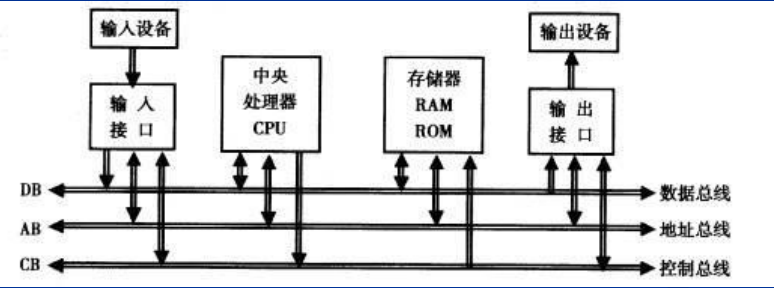
\includegraphics[width=\textwidth]{./images/io_hardware.png}

    \item [(2). ] I/O系统组成成分
    \begin{itemize}
        \item I/O设备:具体完成数据I/O的设备
        \item 设备控制器:负责连接I/O设备和数据总线,完成设备控制和数据格式转换。
        \item I/O通道:目的是使原来由CPU处理的I/O任务转由通道来承担,从而把CPU从繁杂的I/O任务中解脱出来。
    \end{itemize}
    \item [(3). ] I/O系统结构
    \begin{itemize}
        \item 单通路I/O系统:无冗余设备,容错性差
        \item 多通路I/O系统:有冗余设备,容错性好
    \end{itemize}
\end{enumerate}

I/O设备的分类
\begin{itemize}
    \item 按速率分类
    \begin{itemize}
        \item 低速设备(键盘)
        \item 中速设备(打印机)
        \item 高速设备(磁盘)
    \end{itemize}
    \item 按信息交换单位分类
    \begin{itemize}
        \item 字符设备(键盘)
        \item 块设备(磁盘)
    \end{itemize}
\end{itemize}

设备控制器的功能
\begin{itemize}
    \item 接收和识别命令
    \item 数据交换
    \item 标志和报告设备状态
    \item 地址识别
    \item 数据缓冲
    \item 差错控制
\end{itemize}

\subsubsection{I/O控制方式}

主要有四种
\begin{itemize}
    \item 程序I/O方式
    \item 中断驱动I/O控制方式
    \item DMA方式
    \item 通道控制方式
\end{itemize}

\subsection{缓冲管理}

\subsubsection{缓冲的引入}

引入缓冲的原因
\begin{itemize}
    \item 缓和CPU和I/O设备的矛盾;
    \item 减少CPU中断的频率;
    \item 解决数据粒度不匹配的问题;
    \item 提高CPU和I/O设备的并行性。
\end{itemize}

\subsubsection{单缓冲}

引入如下几个时间:
\begin{itemize}
    \item 从磁盘把数据输入到缓冲区的时间为T
    \item OS从缓冲区将数据传送到用户区的时间为M
    \item CPU处理这块数据的时间为C
\end{itemize}

T和C是可以并行的,故单缓冲区条件下,系统对每一块数据的处理时间为Max(C,T)+M。

\subsubsection{双缓冲}

双缓冲时,系统处理一块数据的时间可以粗略认为是Max(C,T)。

\subsubsection{循环缓冲}

略

\subsubsection{缓冲池}

略

\subsection{设备分配}

\subsubsection{设备分配的基本概念}

略

\subsubsection{设备独立性}

定义:用户程序独立于具体使用的物理设备。

实现:引入逻辑设备和物理设备
\begin{itemize}
    \item 逻辑设备:是对一组具备相同功能物理设备的抽象;
    \item 物理设备:应用程序实际执行时,使用的特定类型设备。
\end{itemize}

基本做法:编写程序时,使用逻辑设备名称访问设备;
程序执行时,使用具体的物理设备完成实际数据操作。

为每个用户设置一张逻辑设备表(LUT),完成逻辑设备到物理设备的映射。

设备独立性的优点
\begin{itemize}
    \item 设备分配时的灵活性
    \item 容易实现I/O重定向
\end{itemize}

\subsubsection{SPOOLing技术}

SPOOLing: Simultaneaus Periphernal Operating On-Line,中译名“假脱机”

为了缓和CPU的高速性和I/O设备低速性之间的矛盾,引入脱机输入/输出技术。
多道程序环境下,可以利用其中的一道程序模拟脱机技术中的外围控制机,实现假脱机效果。

典型应用:共享打印机

SPOOLing系统的基本组成
\begin{itemize}
    \item 输入井和输出井
    \item 输入缓冲区和输出缓冲区
    \item 输入进程和输出进程
    \item 井管理程序
\end{itemize}

SPOOLing特点
\begin{itemize}
    \item 提高I/O速度
    \item 改造独占设备为共享设备
    \item 实现了虚拟设备功能
\end{itemize}

\subsection{磁盘存储器的性能和调度}

\subsubsection{磁盘性能概述}

磁盘访问时间
\begin{equation}
    T=T_s+T_r+T_t
\end{equation}

其中
\begin{itemize}
    \item $T_s$:寻道时间
    \item $T_r$:旋转延迟时间
    \item $T_t$:传输时间
\end{itemize}

\subsubsection{早期的磁盘调度算法}

\begin{itemize}
    \item 先来先服务(FCFS)算法:根据进程请求到来的次序进行服务。公平、简单,不会出现长时间得不到相应的情况。但平均寻道距离较大,不适合进程较多的情况。
    \item 最短寻道时间优先(SSTF)算法:访问距离最近的请求磁道,从而最小化寻道时间。有“磁臂粘着”现象。
\end{itemize}

\subsubsection{基于扫描的磁盘调度算法}

\begin{itemize}
    \item 扫描(SCAN)算法:访问距离最近且在当前磁头移动方向上的请求磁道。磁头到达边缘后改变方向折返。有效解决“磁臂粘着”。
    \item 循环扫描(CSCAN)算法:即单向的SCAN,磁头移动到最外磁道后,不是访问最近的请求磁道,而是立即返回最内侧磁道,再向外移动。
\end{itemize}

\newpage
\section{文件管理}

\subsection{文件和文件系统}

文件的定义:文件是指由创建者所定义的、具有文件名的若干相关元素的集合。

\subsubsection{数据项、记录和文件}

在文件系统中,数据项是最低级的数据组织形式。也称字段。可分为
\begin{itemize}
    \item 基本数据项:单个数据项
    \item 组合数据项:由若干个基本数据项组成
\end{itemize}

记录是一组相关数据项的集合,用于描述一个对象在某方面的属性。可分为
\begin{itemize}
    \item 定长记录:记录长度固定
    \item 变长记录:记录长度不定
\end{itemize}

为了唯一标识一个记录,必须从记录的各个数据项中确定一个或多个数据项作为关键字(Key)。

\subsubsection{文件系统的层次结构}

文件管理系统管理的对象:
\begin{itemize}
    \item 文件
    \item 目录
    \item 磁盘存储空间
\end{itemize}

文件系统接口:
\begin{itemize}
    \item 命令接口
    \item 程序接口
\end{itemize}

\subsubsection{文件操作}

最基本的文件操作:
\begin{itemize}
    \item 创建文件
    \item 删除文件
    \item 读文件
    \item 写文件
    \item 设置文件的读/写位置
\end{itemize}

\subsection{文件的逻辑结构}

所有文件都有如下两种形式的结构:
\begin{itemize}
    \item 逻辑结构,这是从用户观点看到的结构,也叫文件组织。
    \item 物理结构,用户不可见。
\end{itemize}

\subsubsection{文件逻辑结构的分类}

按照是否有结构来分:
\begin{itemize}
    \item 有结构文件(记录式文件)
    \begin{itemize}
        \item 定长记录:检索容易
        \item 变长记录:灵活
    \end{itemize}
    \item 无结构文件(流式文件)
\end{itemize}

按照文件的组织方式,将有结构文件分为以下三类:
\begin{itemize}
    \item 顺序文件
    \item 索引文件
    \item 索引顺序文件
\end{itemize}

正规OS:顺序文件+暴露读写指针

\subsubsection{顺序文件}

顺序文件的记录是定长记录或可变长记录。
\begin{itemize}
    \item 最佳应用场合:对文件中的记录进行批量存取时。
    \item 若共有$N$个记录,则查找一个记录平均需要查$N/2$次。即查找性能不好。
    \item 此外添加或删除一个记录也很困难。可以引入一个事务文件,保存一段时间内的新增和删除记录,每隔一段时间进行实际写入。
\end{itemize}

为了访问顺序文件中的记录,必须首先找到记录的地址。有两种方法
\begin{itemize}
    \item 隐式寻址:就是从头找起,无论记录是定长的还是不定长的。
    \item 显式寻址:仅能用于寻址定长记录文件,直接将基址加上偏移量得到,由于定长,偏移量很容易得到。
\end{itemize}

\subsubsection{索引文件}

主要用于解决变长记录文件的快速查找问题。

方法:建立一张索引表,其中保存有每个记录的“指针”,是定长的,这样就可以按照关键字查找索引表,然后再跳转到实际记录。

也可以建立多个索引表,从而支持按照多个属性进行索引。

缺点是索引表须占用额外存储空间,尤其当记录数量很大时。

\subsubsection{索引顺序文件}

顺序文件和索引文件的一种折中。

将记录分组,为每组记录在索引表中建立一个项。

分组方式:按关键字分组,或直接按记录号分组。

查找过程:首先查索引表,找到待查项所在的组,通过指针跳转,再在组中顺序查找。

可以引入多级索引。

\subsubsection{直接文件和哈希文件}

课本和PPT说法不太一样,略了。

\newpage
\section{磁盘存储器的管理}

\subsection{外存的组织方式}

常见方式:
\begin{itemize}
    \item 连续组织方式
    \item 链接组织方式
    \item 索引组织方式
\end{itemize}

\subsubsection{连续组织方式}

为每个文件分配一组相邻接的磁盘块,且文件的逻辑记录
的顺序与所存储磁盘块的块号顺序一致。

优点:
\begin{itemize}
    \item 顺序访问很容易。
    \item 顺序访问速度快。
\end{itemize}

缺点:
\begin{itemize}
    \item 要求为文件分配连续的存储空间,很容易出现碎片。而外存的紧凑代价是难以想象的。
    \item 必须事先知道文件长度,同理,很难处理动态增长的文件。
    \item 不能快速插入和删除记录。
\end{itemize}

\subsubsection{链接组织方式}

为每个文件分配一组不相邻接的磁盘块,
且文件的逻辑记录的顺序与所存储磁盘块的块号顺序可以不一致。

核心问题:如何设计数据结构,来存储文件的所有磁盘块的位置。

两种方法:
\begin{itemize}
    \item 隐式链接法:每个磁盘块设置一个指针指向下一个磁盘块。
    \item 显式链接法:把所有指针存在一张链接表内,即所谓文件分配表FAT(File Allocatin Table),使用时将FAT表载入内存,在内存中查找,从而大大加速。
\end{itemize}

\subsubsection{FAT技术}

引入“卷”的概念,支持将一个物理磁盘分成4个卷(也称分区)。

一个扇区一般是512KB大小。

FAT12
\begin{itemize}
    \item 每个分区保存两张相同的FAT表。
    \item 将文件的第一个盘块号放在自己的FCB中。
    \item 可以将相邻的若干个扇区在逻辑上合并为“簇”(cluster),进一步扩大最大容量。
    \item 支支持8+3格式的短文件名。
\end{itemize}

FAT16:FAT12的简单改进版本

FAT32
\begin{itemize}
    \item 分区容量不大于8GB时,每个簇都固定为4KB。
    \item 分区为8-16GB时,每个簇为8KB。
    \item 分区为16-32GB时,每个簇为16KB
    \item 分区为32GB以上时,每个簇为32KB
    \item 支持长文件名。
    \item 不支持小于512MB的分区,单文件长度不能大于4GB。
    \item 不能向下兼容。
\end{itemize}

\begin{table}[!ht]
    \centering
    \begin{tabular}{|c|c|c|c|}
    \hline
        \textbf{块大小} & \textbf{FAT12} & \textbf{FAT16} & \textbf{FAT32} \\ \hline
        \textbf{0.5KB} & 2MB & ~ & ~ \\ \hline
        \textbf{1KB} & 4MB & ~ & ~ \\ \hline
        \textbf{2KB} & 8MB & 128MB & ~ \\ \hline
        \textbf{4KB} & 16MB & 256MB & 1TB \\ \hline
        \textbf{8KB} & ~ & 512MB & 2TB \\ \hline
        \textbf{16KB} & ~ & 1024MB & 2TB \\ \hline
        \textbf{32KB} & ~ & 2048MB & 2TB \\ \hline
    \end{tabular}
    \caption{FAT中簇的大小与最大分区的对应关系}
\end{table}

\subsubsection{NTFS技术}

略

\subsubsection{索引组织方式}

每个文件分配一个索引表,记录该文件的所有盘块。

优点:支持直接访问,不会产生外部碎片。

缺点:不适合小文件

也可使用多级索引。

\subsection{文件存储空间的管理}

\subsubsection{空闲表法}

系统为外存所有空闲区建立一张空闲表,每个空闲区对应一个空闲表项。

\subsubsection{空闲链表法}

把外存所有空闲区拉成一张空闲盘区(块)表。
\begin{itemize}
    \item 空闲盘块链:结点代表一个空闲盘块
    \item 空闲盘区链:结点代表一个空闲盘区
\end{itemize}

\subsubsection{位视图法}

利用二进制的一位来表示磁盘中一个盘块的使用情况。0表示空闲,1表示占用。



\begin{itemize}
    \item 当从1开始编号时,有:
    \begin{itemize}
        \item 位视图第i行第j列对应的盘块号为
        \begin{equation}
            b=n(i-1)+j
        \end{equation}
        其中n为每行的位数。
        \item 给定盘块号b,按照如下公式对应到位视图:
        \begin{gather}
            i=[(b-1)\text{整除}n]+1 \\
            j=(b-1)\text{MOD}n+1
        \end{gather}
    \end{itemize}
    \item 当从0开始编号时,有:
    \begin{itemize}
        \item 位视图第i行第j列对应的盘块号为
        \begin{equation}
            b=n\times i+j
        \end{equation}
        其中n为每行的位数。
        \item 给定盘块号b,按照如下公式对应到位视图:
        \begin{gather}
            i=b\text{整除}n \\
            j=b\text{MOD}n
        \end{gather}
    \end{itemize}
\end{itemize}

\begin{problem}
    在位视图法中,假如字长为32,则90号磁盘块对应的行号为(\ \ ),列号为(\ \ )。(行号、列号、磁盘块号均从0开始编号)
\end{problem}

\begin{solution}
    \begin{gather*}
        i=90/32=2 \\
        j=90\ \text{MOD}\ 32=26
    \end{gather*}
\end{solution}

\newpage
\section{操作系统接口}

操作系统是人和计算机之间的接口。

操作系统接口是用户和操作系统之间的接口。

分类:
\begin{itemize}
    \item 用户接口:提供给用户。
    \begin{itemize}
        \item 联机命令接口:字符式。用户使用命令语言和OS交互。命令语言包括:
        \begin{itemize}
            \item 命令行方式
            \item 批命令方式
        \end{itemize}
        \item (联机)图形用户接口GUI
        \item 脱机用户接口(用于批处理)
    \end{itemize}
    \item 程序接口:提供给程序。用户程序取得OS服务的唯一途径。
\end{itemize}

\subsection{系统调用}

程序接口是由一组系统调用(system call)组成的。

系统调用是特殊的过程调用,它和一般的过程调用有如下区别:
\begin{itemize}
    \item 运行在不同的系统状态。一般的过程调用的调用者和被调用者运行在同一个状态,而系统调用的调用者运行在用户态,而被调用者运行在系统态。
    \item 状态的转换。一般的过程调用不涉及状态转换,系统调用涉及从用户态到系统态的转换,这是通过软中断机制实现的。
    \item 嵌套调用,系统调用可以嵌套,但一般都有最大深度限制,而一般的过程调用则没有限制。
\end{itemize}

系统调用的实现:
\begin{itemize}
    \item 在操作系统中,每个系统调用都对应一个事先给定的功能号,例如0、1、2、3等。
    \item 在陷入指令中必须包括对应系统调用的功能号。有些陷入指令中,还带有传给陷入处理机构和内部处理程序的有关参数。
    \item 为实现系统调用功能的子程序编造入口地址表,每个入口地址与相应的系统程序对应。
\end{itemize}

系统调用的过程:
\begin{itemize}
    \item 将处理机状态从用户态转为系统态。
    \item 由硬件和内核程序进行系统调用的一般性处理,包括保护进程的CPU环境和传递用户定义的参数。
    \item 分析系统调用的类型,转入相应的系统调用处理程序。
    \item 系统调用处理程序执行完后,恢复CPU现场,返回被中断进程,继续执行。
\end{itemize}

\end{document}